\documentclass[tikz]{standalone}
\usetikzlibrary{calc,arrows}

\begin{document}
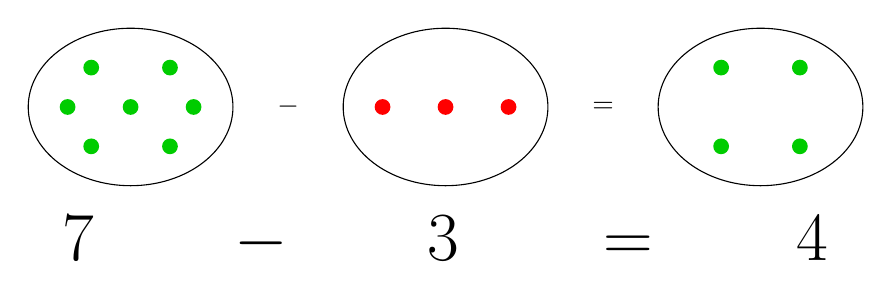
\begin{tikzpicture}
    \draw (0,0) circle (1.3 and 1);
    \node at (2,0) {$-$};
    \draw (4,0) circle (1.3 and 1);
    \node at (6,0) {$=$};
    \draw (8,0) circle (1.3 and 1);

    \fill[green!80!black] (0,0) circle (0.1);
    \fill[green!80!black] (0.5,0.5) circle (0.1);
    \fill[green!80!black] (-0.5,0.5) circle (0.1);
    \fill[green!80!black] (0.8,0) circle (0.1);
    \fill[green!80!black] (-0.8,0) circle (0.1);
    \fill[green!80!black] (0.5,-0.5) circle (0.1);
    \fill[green!80!black] (-0.5,-0.5) circle (0.1);

    \fill[red] (4,0) circle (0.1);
    \fill[red] (4.8,0) circle (0.1);
    \fill[red] (3.2,0) circle (0.1);

    \fill[green!80!black] (8.5,0.5) circle (0.1);
    \fill[green!80!black] (7.5,0.5) circle (0.1);
    \fill[green!80!black] (8.5,-0.5) circle (0.1);
    \fill[green!80!black] (7.5,-0.5) circle (0.1);

    \node at (4,-1.7) {\Huge $7~~~~~~-~~~~~~3~~~~~~=~~~~~~4$};
\end{tikzpicture}
\end{document}